\documentclass[tikz]{standalone}
\usepackage{pgfplots}
\pgfplotsset{compat=1.15}
\usepackage{mathrsfs}
\usetikzlibrary{arrows,calc}
\usepackage{tkz-euclide}
\pagestyle{empty}

\definecolor{AngleClr}{rgb}{0,0.39215686274509803,0}
\definecolor{ShapeClr}{rgb}{0.6,0.2,0}
\definecolor{BlueClr}{RGB}{250, 248, 217}


\begin{document}

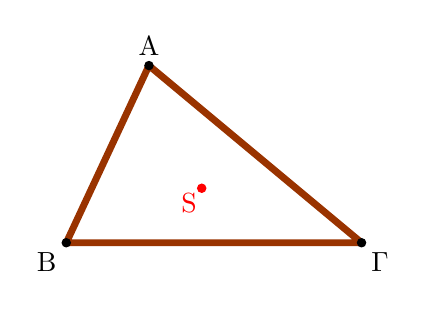
\begin{tikzpicture}[scale=.75]
\tkzSetUpLine[line width=1pt,color=black]
\tkzSetUpPoint[fill=black]

\tkzDefPoints{0/0/B,1.4/3/A,5/0/C}

\tkzDefMidPoint(B,C) \tkzGetPoint{MA}
\tkzDefMidPoint(A,C) \tkzGetPoint{MB}
\tkzDefMidPoint(A,B) \tkzGetPoint{MC}


\tkzInCenter(MA,MB,MC)\tkzGetPoint{S}
\tkzDefPointBy[projection=onto MA--MB](S)\tkzGetPoint{P}

\tkzInterLL(B,MB)(C,MC)
\tkzGetPoint{G}

\tkzDrawPolygon[color=ShapeClr,line width=2.5pt](A,B,C)

\tkzDrawPoints[size=3](A,B,C)
\tkzDrawPoints[size=3,red](S)

\tkzLabelPoint[above](A){$\rm A$}
\tkzLabelPoint[below left](B){$\rm B$}
\tkzLabelPoint[below right](C){$\rm \Gamma$}

\tkzLabelPoint[below left,xshift=0.18cm,red](G){$\rm S$}

\end{tikzpicture}
\end{document}
